 \newcommand{\pwd}{key}

\renewcommand{\password}{key\xspace}

We introduce the problem  through an example, and outline our
approach.  We work with a  small, class-based object-oriented, sequential language similar to Joe-E \cite{JoeE} with modules,   module-private fields
({accessible} only from   methods {from} the same module),
and unforgeable, un-enumerable addresses.
We distinguish between  \emph{\internalO  objects} --- instances of our internal module $M$'s classes ---
and \emph{\externalO  objects} defined in
\emph{any} number of external modules $\overline M$\footnote{We use the notation $\overline z$ for a sequence of $z$, \ie for $z_1,z_2,...z_n$ }.~ 
States whose receiver (\prg{this}) is internal are \emph{internal states} -- they are executing code from the internal module -- the other states are  \emph{external states}.
{\prg{Private} methods  {may only be} called by objects of the same
  module,  while \prg{public}  methods  may be \sue{called} by \emph{any}
  object with a reference to the method receiver, {and with
  actual arguments of  dynamic types that match} the declared formal parameter types.} 
\footnote{As in Joe-E, we leverage  module-based privacy to restrict propagation of capabilities, and reduce the need for reference monitors etc, \cf Sect 3 in  \cite{JoeE}.}   

 \label{s:concepts}
 
We are concerned with guarantees made in an \emph{open} setting; % thatis, 
Our internal module
$M$ must be programmed so that 
  execution of $M$  together with \emph{any} unknown, arbitrary, external modules $\overline M$
% it was "its execution, together ... "SD thinks that the comma  was misleading
will satisfy these guarantees --
%$M$ must ensure these guarantees are satisfied
%These guarantees must  satisfied whenever the $\overline M$  \emph{\externalM} modules are executing, yet 
without relying on any assumptions about $\overline M$'s code
(beyond the programming language's semantics) 
\footnote{
This is a critical distinction from e.g.\
cooperative approaches such as rely/guarantee
\cite{relyGuarantee-HayesJones-setss2017,relyGuarantee-vanStaden-mpc2015}.}.
% SD chopped the next sentence. Because I think that  the uninformed reader will be surpised, and the knowledgeable reader will find out soon enough
% The internal module may break these guarantees temporarily,
% so long as they {are reestablished} before (re)entry to an external module.
  
 

\subsection*{\prg{Shop} -- illustrating limited effects}  
\label{sec:how}
\label{sec:shop}

Consider the following, internal, module \Mshop, % which also includes the 
containing classes \prg{Item}, \prg{Shop}, \prg{Account}, and \prg{Inventory}. 
Classes  {\prg{Inventory} and \prg{Item} have the expected functionality. 
\prg{Account}s hold a balance and have a \password. 
Access to an \prg{Account},  allows one  to pay money into it, 
and  access to an \prg{Account}  and its \prg{Key}, allows one to withdraw money from it.
% Implementations of such a class  appear in the next section.
}
 \prg{Shop}  has  a public method \prg{buy} whose formal parameter \prg{buyer} is an \prg{external}   object. 
 % SD chopped  with a method { \prg{pay}.}} 

\begin{lstlisting}[mathescape=true, language=Chainmail, frame=lines]
module M$_{shop}$
  ...   
  class Shop
    field accnt:Account, invntry:Inventory, clients:external      
    public method buy(buyer:external, anItem:Item)
      int price = anItem.price
      int oldBlnce = this.accnt.blnce
      $\red{\mbox{buyer.pay(this.accnt, price)}}$      
      if (this.accnt.blnce == oldBlnce+price)  
         this.send(buyer,anItem)
      else
         buyer.tell("you have not paid me")      
    private method send(buyer:external, anItem:Item)  
       ...         
\end{lstlisting}
 
 

The   sketch below  shows a possible heap snippet. Red and green rounded rectangles indicate external and internal objects, respectively. 

\noindent
\begin{flushleft}
\begin{tabular}{@{}lll@{}}
  \begin{minipage}{.74\textwidth}
Each object has a  number, % (address), 
 followed by an abbreviated class name. Here, $o_1$, $o_2$ and $o_5$ are a \prg{Shop}, an \prg{Inventory}, and an external object. 

Curved arrows %between objects 
indicate field values. Here, $o_1$ has three fields, pointing to 
$o_4$, $o_5$ and $o_2$.
%
Fields denote direct access. The transitive closure of direct access gives indirect (or transitive) access. Here, $o_1$ has direct access to $o_4$, and indirect access to $o_6$.

Object $o_6$ is %the key to the account $o_4$, and represents 
the capability that allows withdrawal from $o_4$. We highlight this through a dark outline to $o_6$.
\end{minipage}
& \ \  \   &
\begin{minipage}{.25\textwidth}
%\begin{figure}
% I wanrted a figure here, but it went soemwhere else
\resizebox{2.2cm}{!}{
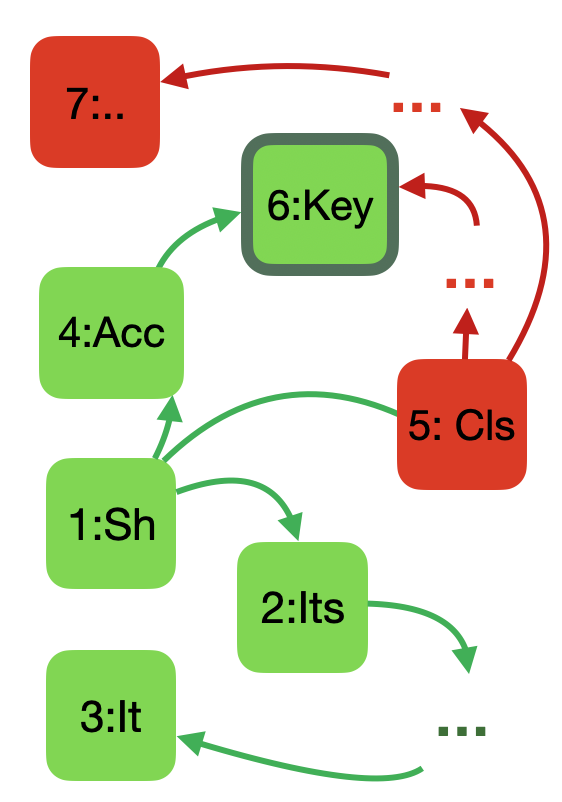
\includegraphics[width=\linewidth]{diagrams/ShopA.png}
} 
%\caption{A Heap}
%\label{f:heap}
%\end{figure}
\end{minipage}
\end{tabular}
\end{flushleft}

\vspace{.1in}

The critical point in our code is the external call on line 8,   {where the \prg{Shop} asks the \prg{buyer} to pay the price of that item,
by calling  \prg{pay} on \prg{buyer} and passing the \prg{Shop}'s account as an argument.
% somebody had written " \prg{Shop}'s account" but SD thinks it has to be  \prg{Shop}'s account
As \prg{buyer} is an external object, the module \Mshop has no method specification for \prg{pay}, and no 
certainty about what its implementation %knowledge of what the implementation of \prg{pay} 
might do. 
% \se{with \prg{this.accnt}}.  % SD: no, because  also with other things.
}

{What are the possible effects of that external call?}
{The \prg{Shop} hopes, % but cannot be sure,
 that at line 9  it  will have received money; but 
it wants to be certain  that the \prg{buyer} cannot use this opportunity to access the 
shop's account to drain its money.

Can \prg{Shop}  be certain?} Indeed, if

\vspace{.05cm}
\begin{enumerate}[(A)]
\item   Prior to the call of  \prg{buy}, the \prg{buyer}  has no eventual access to the account's \password, \ \ \ \emph{----} and
\item  \Mshop ensures that 
\begin{enumerate}[(a)]
\item access to keys is not leaked to external objects, \ \ \ \emph{----} and
\item   funds cannot be withdrawn unless the external entity responsible for the withdrawal has eventual access to the account's \password,
\end{enumerate}
\ \  \ \ \ \emph{----} then
\item  The external  call on line 8 will not result  in a decrease in the shop's account balance.
\end{enumerate}



%\vspace{.3cm}
\noindent
The remit of this paper is to provide specification and verification tools that support arguments like the one above.
This gives rise to the following three challenges:\  1$^{st}$:  A specification language which describes access to capabilities and limited effects,\ 
2$^{nd}$: A  Hoare Logic for adherence to such specifications,  \ 3$^{rd}$:    A  Hoare Logic for external calls.

%\begin{description}
%\item[\ \ \ \ \  1$^{st}$ Remit:]  \ A specification language which describes access to capabilities and limited effects,
%
%\item[\ \ \ \ \   2$^{nd}$ Remit:]  A  Hoare Logic for adherence to such specifications,
%
%\item[\ \ \ \ \  3$^{rd}$ Remit:]  A  Hoare Logic for external calls.
%\end{description}

%We continue our example with three versions of the module, some of which satisfy (B) from above, and some of which do not

% In our example, we relied on two yet-to-be-defined concepts: (1) ``eventual access'' and (2) limited effects (e.g., no money withdrawn unless certain conditions are met).
%Therefore, we need to address the following three challenges: 
%\begin{description}
%\item[\ \ \ \ \  1$^{st}$ Challenge] The specification   of ``eventual  access''. 
%
%\item[\ \ \ \ \   2$^{nd}$ Challenge] The specification of limited effects, 
%
%\item[\ \ \ \ \  3$^{rd}$ Challenge] A  Hoare Logic for external calls, and for adherence to limited effect specifications.
%\end{description}



%\vspace{.2cm}
%\noindent
% \textbf{NOTE}  \sdN{Replacing the argument by a wrapper to the account which allows payments but forbids withdrawals,    would be ineffectual in \taming} the  effects on line 9. 
%What  if the   \prg{buyer} had access to the account and its \password  \emph{before} the call to \prg{pay}? 
%\se{I don't understand the point here. Are you saying a wrapper might prevent a buyer who has legitimate access to an account from getting it?}
%\sdN{SD: The point I am trying to make is that: \  if before the call to \prg{pay}, the \prg{buyer} had access to the account and its keyword, and when we call \prg{pay} instead of 
%\prg{this.accnt} we pass the wrapper, then the \prg{buyer} would still be able to steal money from \prg{this.accnt}.
%Does this make sense? Shall we drop that point?}
 
 
\subsection{1$^{st}$ Challenge: Specification Language} 

We want to give a formal meaning to the guarantee that for some effect, $E$, and an object $o_c$ which is the capability for $E$:

\vspace{.1cm}

  \begin{minipage}{.05\textwidth}
   \textbf{(*)}
\end{minipage}
\hfill
\begin{minipage}{.95\textwidth}
\begin{flushleft}
$E$ \sue{(\eg the account's balance decreases)} can be caused only  by external objects calling methods on internal objects, \\
and only if the causing object has access  to $o_c$ \sue{(\eg the key)}. 
\end{flushleft}
\end{minipage}

\vspace{.1cm}

%\begin{quote}
%(*)   \ \ \ \ \ $E$ can be caused only  by external objects calling methods on internal objects, \\
%$\strut \ $ \ \ \ \ \  \ \ \ and only if the causing object has access  to $o_c$.   
% \end{quote}

\noindent 
The first task is to describe that effect  $E$ took place: if we  find  some assertion $A$ \sue{(\eg must have the key to lower the balance)}which is invalidated by $E$, then, (*) can be described by something like:

\vspace{.1cm}

  \begin{minipage}{.05\textwidth}
   \textbf{(**)}
\end{minipage}
\hfill
\begin{minipage}{.95\textwidth}
\begin{flushleft}
If $A$ holds, \  and \     no external access to  $o_c$ \ \ \ \ then\  \ \  \ $A$ holds in the future. 
\end{flushleft}
\end{minipage}

\vspace{.1cm}


\noindent 
We next make more precise that "no external access to  $o_c$", and that "$A$ holds in the future".

In a first attempt, we could say that "no external access to  $o_c$" means  that no external object exists, nor will any external objects be created.
 However, this is too strong; it defines away the problem we are aiming to solve.

In a second attempt, we could say that "no external access to  $o_c$" means that no external object has access to $o_c$, nor will ever get access to $o_c$. This is also too strong, as it would preclude $E$ from ever happening, while our remit is that $E$ may happen but only under certain conditions. 

This discussion indicates that the lack of external access to $o_c$ is not a global property, and that the future in which  $A$ will hold is not permanent. 
Instead, they are both defined \emph{from the perspective of the current point of execution}.

Thus:


\vspace{.1cm}

  \begin{minipage}{.05\textwidth}
   \textbf{(***)}
\end{minipage}
\hfill
\begin{minipage}{.95\textwidth}
\begin{flushleft}
\ If $A$ holds, \  and \  no external object  \emph{reachable from the current point of execution}  has access to $o_c$, \\  
\   and\   no  internal objects pass $o_c$ to external objects,  \\
\ then \ \ \  \ $A$ holds in  \emph{the future scoped by the current point of execution}.  
\end{flushleft}
\end{minipage}

\vspace{.2cm}
 
\noindent 
We formalize the concepts "reachable from the current point of execution" and  "future scoped by the current point of execution"
through the concept of \emph{protection}, and \emph{scoped invariants}. 
We discuss these concepts in more detail in \S \ref{sect:approach:protection}, and \S \ref{sect:approach:scoped}.
But first, we clarify the concept of "current point of execution".

\subsubsection*{The Current Point of Execution} is characterized by the heap, and   the activation frame of the currently executing method. 
 Activation frames, or frames for short, consist of a variable map and a continuation -- the statements remaining to be executed. 
Upon method call and return, frames are pushed onto/popped from the call stack.
Thus, the frame on top of the stack is the one most recently pushed; it corresponds to the currently executing method.
\begin{figure}[tbh]
\begin{tabular}{|c|c|c|}
\hline
\resizebox{3.5cm}{!}{
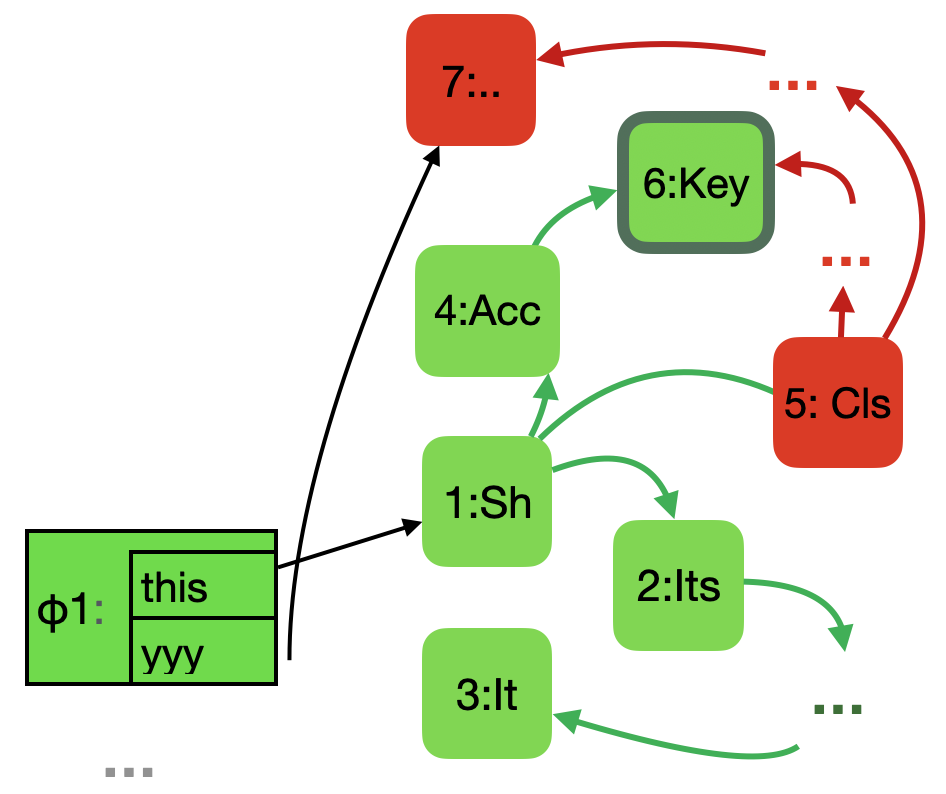
\includegraphics[width=\linewidth]{diagrams/ShopB.png}
} 
&
\resizebox{3.5cm}{!}{
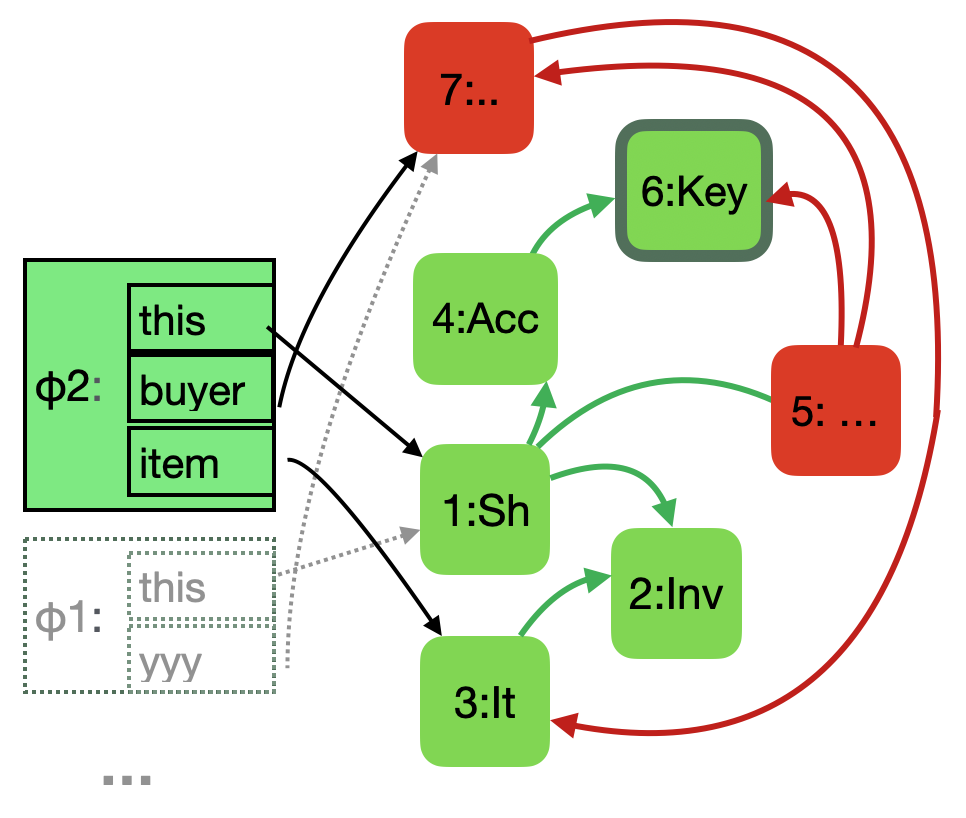
\includegraphics[width=\linewidth]{diagrams/ShopC.png}
}
&
\resizebox{3.5cm}{!}{
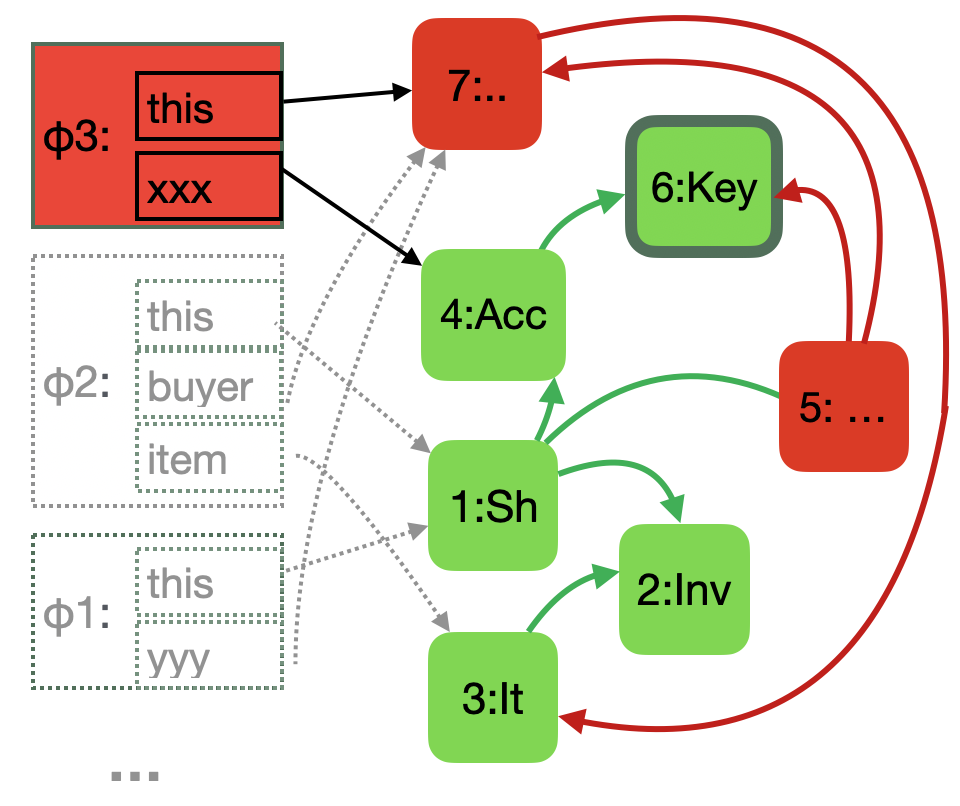
\includegraphics[width=\linewidth]{diagrams/ShopD.png}
}
\\
\hline
$\sigma_1$, top frame $\phi_1$ 
&
$\sigma_2$, top frame $\phi_2$
&
$\sigma_3$, top frame $\phi_3$
\\
\hline % \hline
\end{tabular}
\caption{\textit{ Current point of execution} before \prg{buy}, during \prg{buy}, and during \prg{pay}.  Frames $\phi_1$, $\phi_2$ in green, as their receiver (\prg{this}) is internal;  $\phi_3$ in red as its receiver is external. Continuations were omitted.}
 \label{f:CurrentPoint}
\end{figure}


Fig. \ref{f:CurrentPoint} illustrates these concepts.  The left pane, $\sigma_1$, shows a state with the same heap as earlier, but where the top frame is $\phi_1$ -- it could be the state before a call to \prg{buy}.
  The middle pane, $\sigma_2$, is a state where we have pushed  $\phi_2$ on top of the stack of $\sigma_1$ -- it could be a state during execution of \prg{buy}.
   The right pane, $\sigma_3$, is a state where we have pushed  $\phi_3$ on top of the stack of $\sigma_1$ -- it could be a state during execution of \prg{pay}. 




\subsubsection{Protection}
\label{sect:approach:protection}


 \begin{description}
\item[Protection] 
Object $o$ is \emph{protected  from} $o'$, formally $\protectedFrom {o} {o'}$,  
if no external object transitively accessible from $o'$ has direct access to $o'$.
\\
Object $o$ is \emph{protected}, formally ${\inside{\prg{\it{o}}}}$,  
if no external object transitively accessible from the current frame\footnote{An object is transitively accessible from a frame if
 there exists a sequence of field accesses leading from one of the variables in the frame  to that object.} has direct access to $o$,
 and   if $o$ is not an argument if the receiver is external. 
 
 More in Def. \ref{def:chainmail-protection-from}. % and Fig. \ref{fig:ProtectedBoth}.   
 \end{description}
\sue{ SEVERAL CHANGES. NOTE the last o in the first sentence should not have a '

Object $o$ is \emph{protected  from} $o'$, formally $\protectedFrom {o} {o'}$,  
if no external object transitively accessible from $o'$ has direct access to $o$.
Object $o$ is \emph{protected}, formally ${\inside{\prg{\it{o}}}}$,  
if no external object transitively accessible from the current frame\footnote{An object is transitively accessible from a frame if 
there exists a sequence of field accesses leading from one of the variables in the frame  to that object.} has direct access to $o$,
 and  if the receiver is external then $o$ is not an argument. 
 More in Def. \ref{def:chainmail-protection-from}. % and Fig. \ref{fig:ProtectedBoth}.   

 }
 
 

\begin{figure}[htb]
\begin{tabular}{|c|c|c|c|}
\hline
 & & & 
\\
\resizebox{2.0cm}{!}{
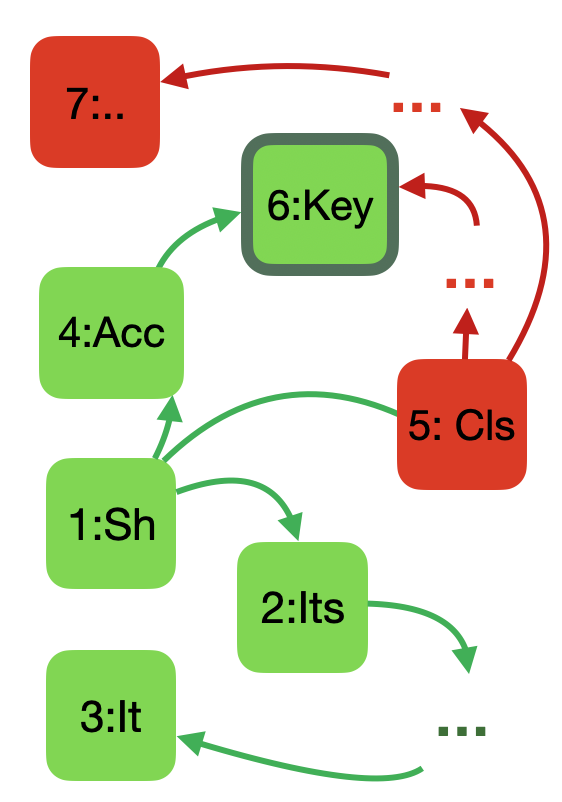
\includegraphics[width=\linewidth]{diagrams/ShopA.png}
} 
&
\resizebox{3,5cm}{!}{
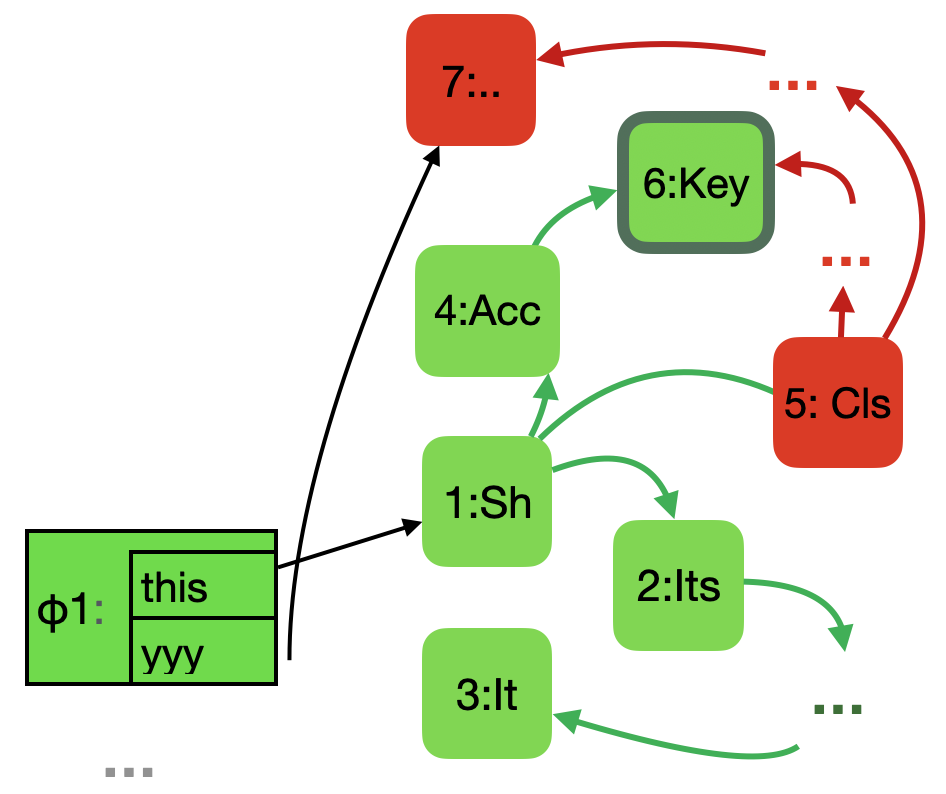
\includegraphics[width=\linewidth]{diagrams/ShopB.png}
} 
&
\resizebox{3,5cm}{!}{
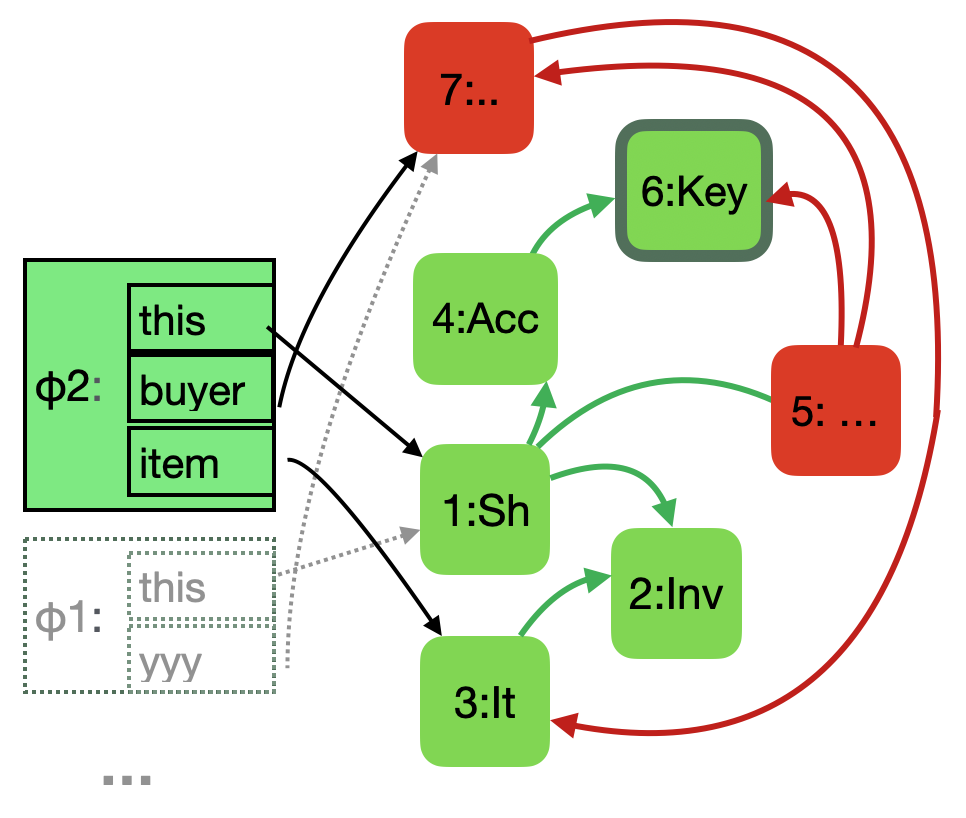
\includegraphics[width=\linewidth]{diagrams/ShopC.png}
}
&
\resizebox{3.5cm}{!}{
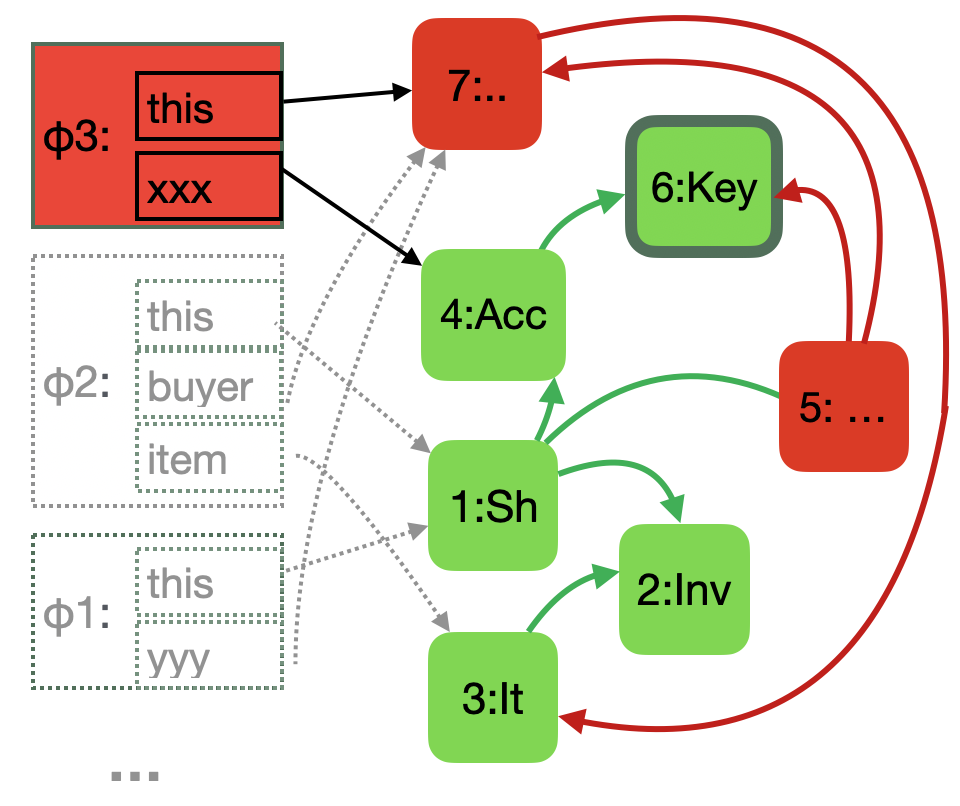
\includegraphics[width=\linewidth]{diagrams/ShopD.png}
}
\\
\hline
 heap
&
$\sigma_1$  % protected from object $o_2$
&
$\sigma_2$ 
&
$\sigma_3$ 
\\
\hline 
$... \models \protectedFrom {o_6} {o_4}$
&
$\sigma_1   \not\models \inside{o_6}$
&
$\sigma_2   \not\models \inside{o_6}$
&
$\sigma_3 \models \inside{o_6}$
\\
$... \not\models  \protectedFrom {o_6} {o_5}$
&
$\sigma_1  \models \inside{o_4}$
&
$\sigma_2 \models \inside{o_4}$
&
$\sigma_3 \not \models \inside{o_4}$
%\\
%$... \not\models  \protectedFrom {o_3} {o_5}$
%& & & 
%\\
%$...  \models  \protectedFrom {o_2} {o_5}$
%& & & 
\\
\hline % \hline
\end{tabular}
\caption{\textit{Protected from and Protected}. -- continuing from Fig, \ref{f:CurrentPoint}.
 }
   \label{fig:ProtectedBoth}
 \end{figure}
 \sue{AFTER 'new top frame' THE SUBSRIPT SHOULD BE 4 NOT 5}
  Fig. \ref{fig:ProtectedBoth} illustrates these concepts. In particular, $o_6$ is not protected in $\sigma_1$ nor $\sigma_2$, but is protected in $\sigma_3$. This is so, because pushing a frame makes fewer objects  transitively accessible from the new top frame -- here, $o_5$ is transitively accessible from the  top frame in $\sigma_2$, but not transitively accessible from the   top frame in $\sigma_3$.
 Moreover, $o_4$  is  protected in $\sigma_1$ and  $\sigma_2$,  and not  protected in $\sigma_3$. 
 This is so, because even though neither $o_5$ nor $o_7$ have direct access to $o_4$, in $\sigma_3$  the receiver is external, and $o_4$ is one of the arguments.


 If the  internal module  never passes $o$ to  external objects (\ie never leaks $o$) and  $o$ is protected, then $o$ will remain protected during execution of the current method and all the methods \emph{it} calls.
However, it need not be protected during execution of the method calling the current method, nor after termination of the current method.   
This discussion leads us to  scoped invariants.
%Going back to the original question, if $o_{c}$ is protected,  and $o_{c}$ is never leaked to external objects, 
%then  effect  $E$ is guaranteed not to occur. % , \se{unless caused by internal code}.



 
%\begin{figure}[tbh]
%\begin{tabular}{|c|c|c|}
%\hline
%\resizebox{3.5cm}{!}{
%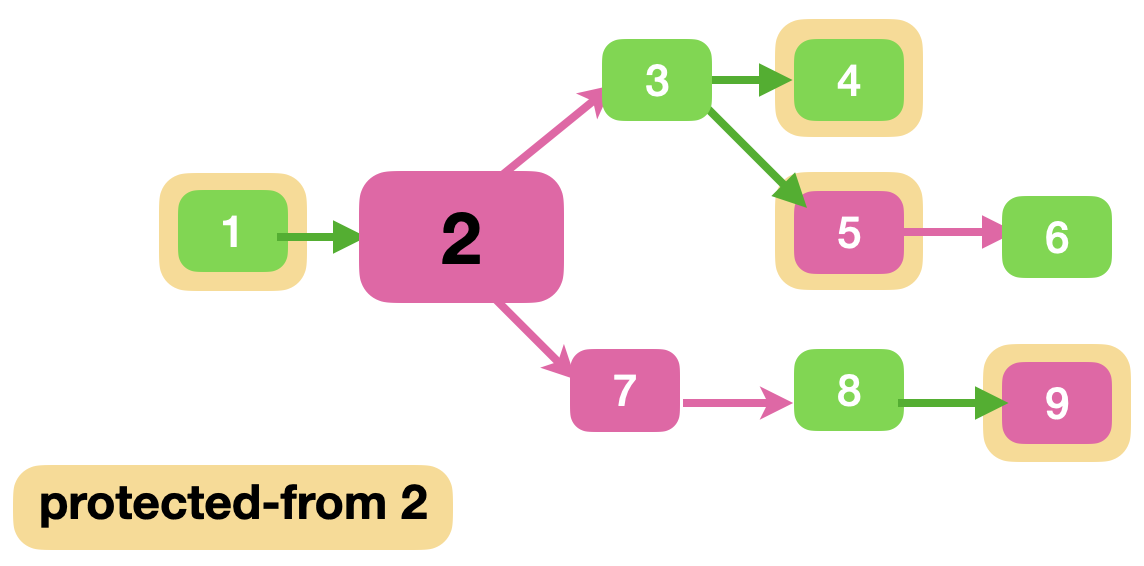
\includegraphics[width=\linewidth]{diagrams/prfC.png}
%} 
%&
%\resizebox{4.5cm}{!}{
%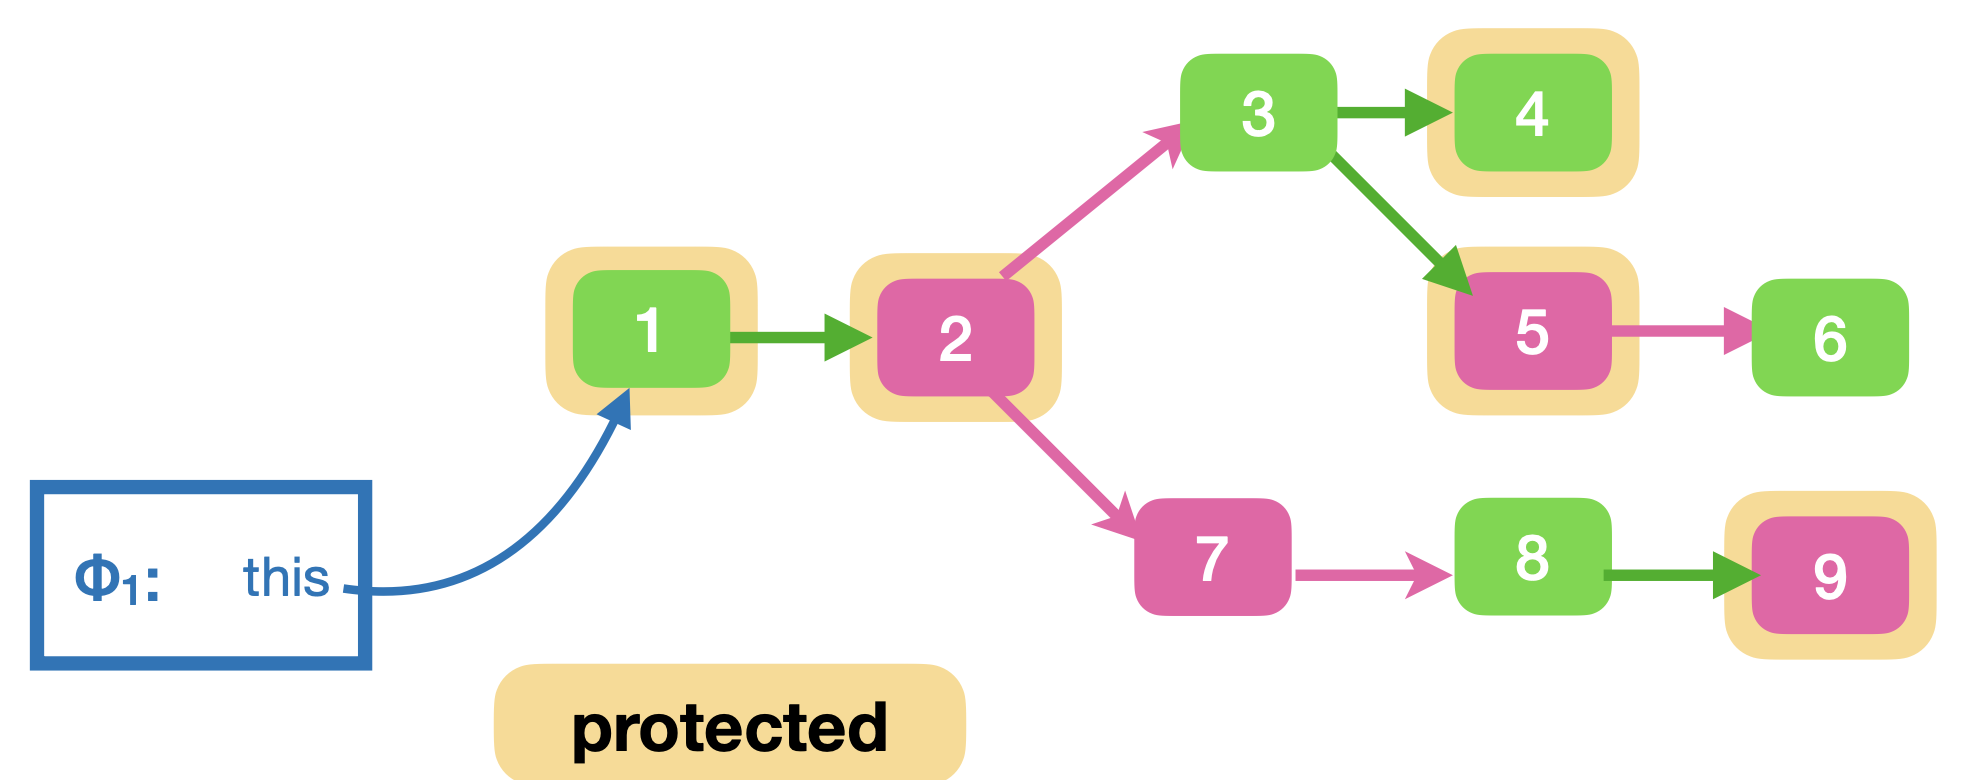
\includegraphics[width=\linewidth]{diagrams/prtFirst.png}
%}
%&
%\resizebox{4.5cm}{!}{
%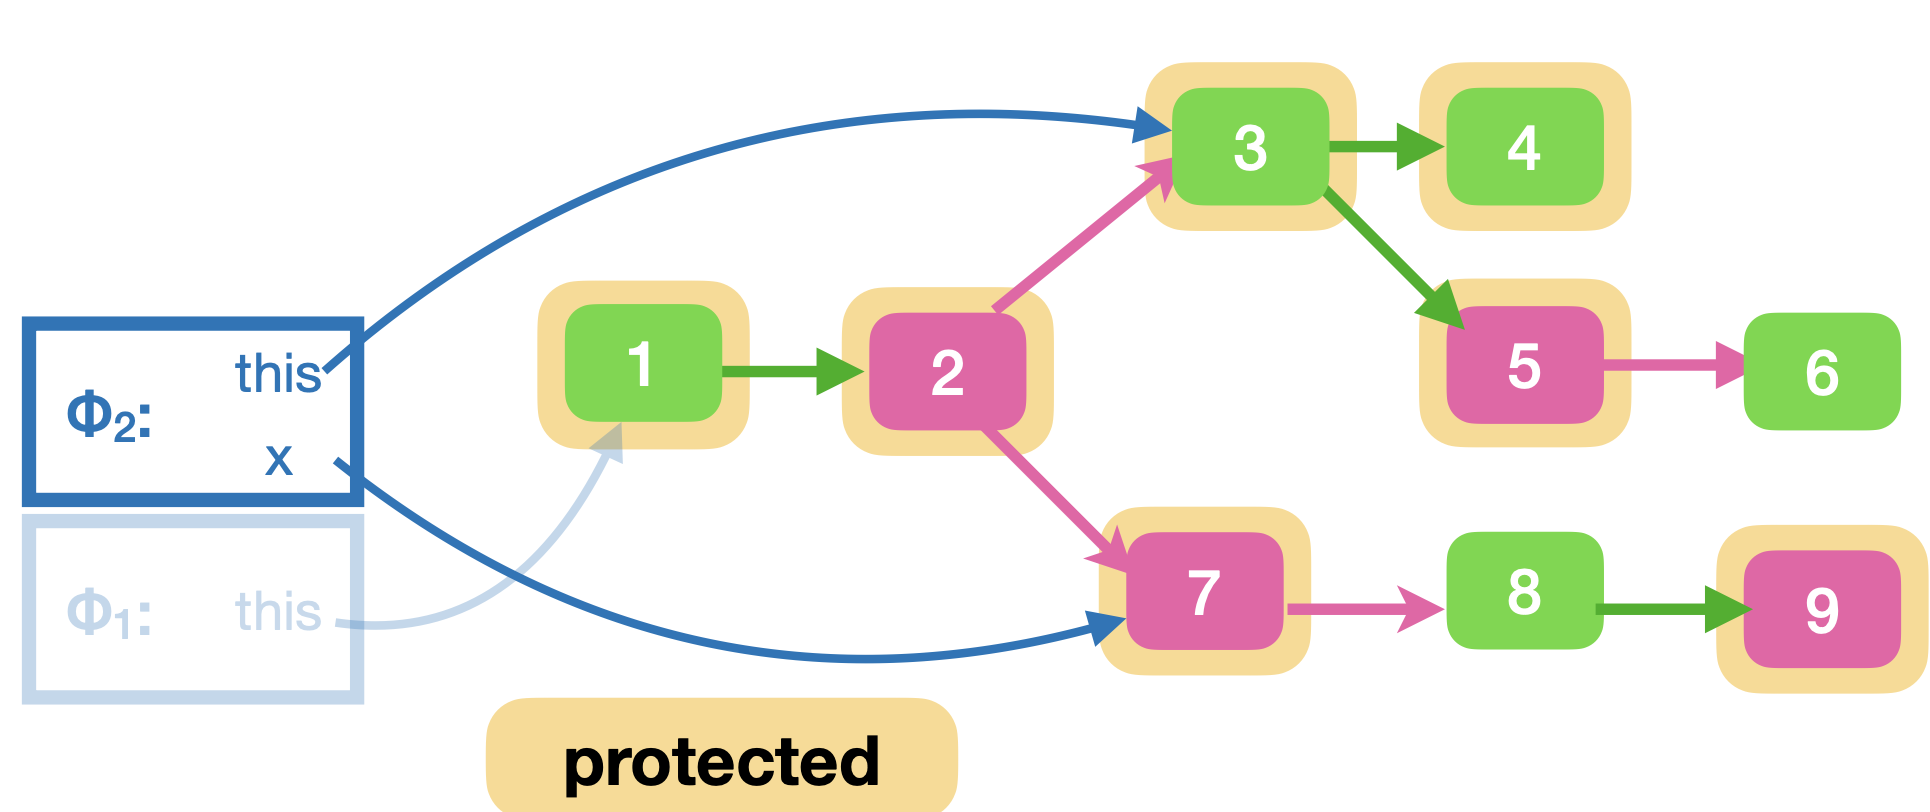
\includegraphics[width=\linewidth]{diagrams/prtSecond.png}
%}
%\\
%\hline
%protected from object $o_2$
%&
%protected  with current frame $\phi_1$
%&
%protected  with current frame $\phi_2$
%\\
%\hline \hline
%\end{tabular}
%\caption{\textit{Protected from and Protected}. Pink and green squares are external and internal objects, respectively. Connecting straight arrows  indicate fields. Blue boxes are frames on the stack. Protected objects are  highlighted in yellow. 
% The left pane shows a heap with objects $o_1$-$o_9$.
% Here  $o_1$, $o_4$, $o_5$ and $o_9$ 
%are protected from $o_2$. 
% The middle pane {shows the same heap and a stack with frame  $\phi_1$} whose receiver,   \prg{this},  points to $o_1$. Here 
% $o_1$, $o_2$, $o_4$, $o_5$ and $o_9$  are protected. 
% The right pane {shows the configuration after pushing frame  $\phi_2$}, whose receiver,  \prg{this},  and local variable, \prg{x}, point to $o_3$ and  $o_7$, respectively.
% Here $o_3$ and $o_7$ are protected, in addition  to  the objects protected in the previous pane.
%}
%   \label{fig:ProtectedBoth}
% \end{figure}
 

\subsubsection{Scoped Invariants}
%\subsection{2$^{nd}$ Challenge: Specification of limited effects}

\label{sect:approach:scoped}
%How can we express the guarantee that effects are limited?  
% In particular, when effects can be the outcome of the execution of more than one method? 
% Traditional,  {per-method} PRE/POST conditions {cannot guarantee} %specifications cannot express guarantees
%  that two or more of our methods won't interact to produce an unlimited effect. 
We build on the concept of history invariants \cite{liskov94behavioral,usinghistory,Cohen10} and define:

\begin{description}
\item[{Scoped invariants}]  
{$\TwoStatesN  {\overline{x:C}}  {A}$} expresses that if an external {state} $\sigma$ 
 has objects $\overline x$ of class $\overline C$, and satisfies $A$, then all $\sigma$'s  {external}, \emph{scoped  future  states}   will  {also} satisfy  {$A$}. 
The scoped future contains all  states which can be reached through any steps, including further method calls and returns, but stopping before returning  from the call active in $\sigma$ \footnote{{Here lies the difference to history invariants, which consider \emph{all} future states, including returning from the call active in $\sigma$.}}  --  \cf Def  \ref{def:shallow:term}.
% {For} $\sigma$ and its scoped future we 
\sdred{Scoped invariants consider external states} only -- \cf Def \ref{def:necessity-semantics}.
\end{description}

 Fig. \ref{fig:illusrPreserve} shows the  states of some, unspecified, execution,   and distinguishes between steps within the same method ($\rightarrow$),
method call ($\uparrow$), and method return ($\downarrow$). %  method; up-arrows represent ; down-arrows represent method returns.
The scoped future of $\sigma_6$ includes all states in the diagram. The scoped future of $\sigma_8$ consists of $\sigma_9$, $\sigma_{10}$,  $\sigma_{11}$,  
$\sigma_{12}$,   $\sigma_{13}$,  and $\sigma_{14}$, and does not include, \eg,  $\sigma_{15}$, or $\sigma_{19}$.
 
 \begin{figure}[htb]
\begin{tabular}{|c|}
\hline  % \\
\hspace{2cm}
\resizebox{7.6cm}{!}{
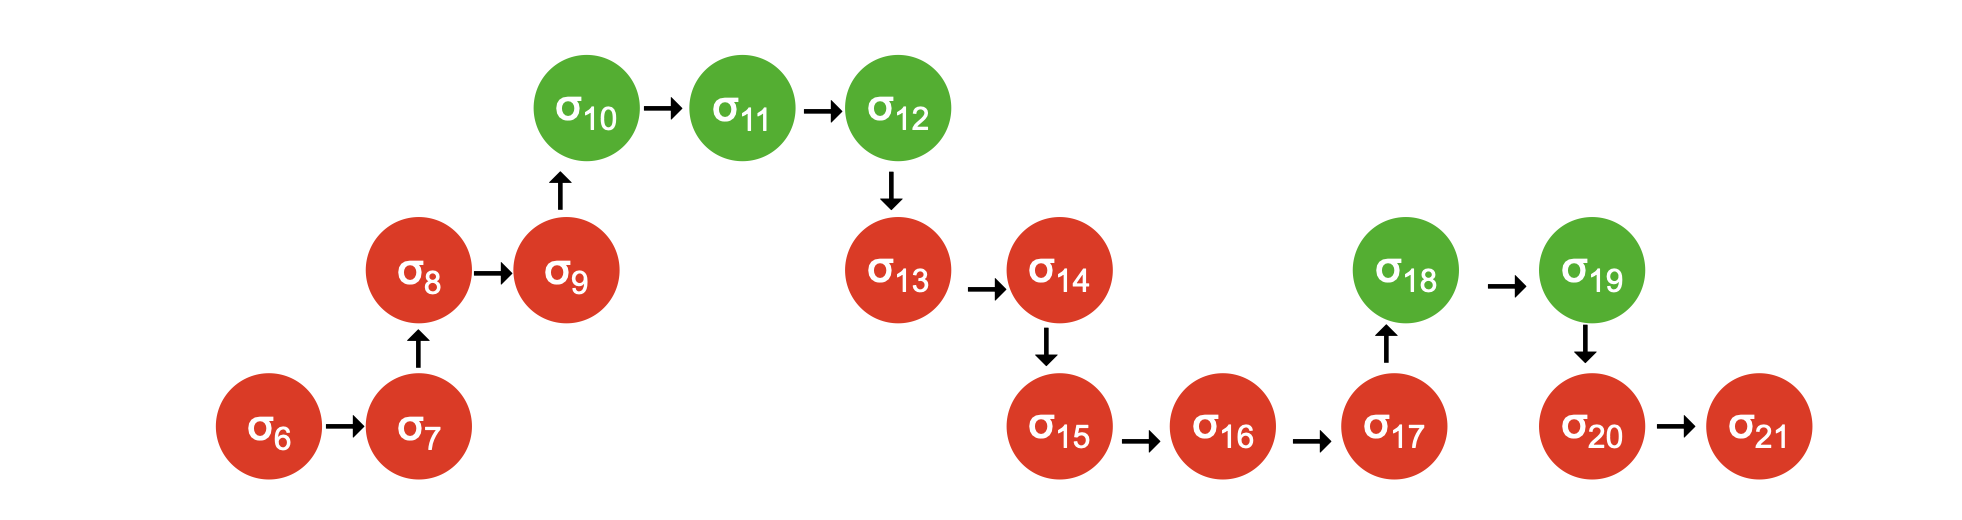
\includegraphics[width=\linewidth]{diagrams/preserve2.png}  % diagrams/preserves2.png} is same but with pink external states
}
\hspace{2cm}
\\
\hline
\end{tabular}
   \caption{ \textit{Execution}.
Green resp. red  disks represent  internal resp. external states.
}
 \label{fig:illusrPreserve} 
 \end{figure}
 
The scoped invariant   ${\TwoStatesN {\overline {x:C}} {A_0}}$   guarantees that  if $A_0$ holds in $\sigma_8$, then it will also hold in $\sigma_9$,    $\sigma_{13}$, and $\sigma_{14}$;
 it %may or may not 
 doesn't have to hold in $\sigma_{10}$, $\sigma_{11}$,  and $\sigma_{12}$ as these are internal states.
Similarly, it guarantees that if $A_0$ holds at $\sigma_6$, then it will also hold at 
$\sigma_7$, $\sigma_8$, $\sigma_9$, $\sigma_{13}$,  $\sigma_{14}$,   $\sigma_{15}$,  $\sigma_{16}$, $\sigma_{17}$,   $\sigma_{20}$ and  $\sigma_{21}$; it may or may not hold at
$\sigma_{10}$, $\sigma_{11}$,  $\sigma_{12}$,  $\sigma_{18}$,  $\sigma_{19}$, as these are internal states.


 

\subsubsection{Examples}    
    
\label{s:bank}

\begin{example}
\label{s:bankSpecEx}
The following scoped invariants\\
$\strut \SPSP\ \ \   S_1\ \  \triangleq \ \ \TwoStatesN {\prg{a}:\prg{Account}}  {\inside{\prg{a}}} $ 
\hspace{1.1cm}
$\strut  \SPSP\ \ \   S_2\ \  \triangleq \ \ \TwoStatesN  {\prg{a}:\prg{Account}}  {\inside{\prg{a.key}}} $ 
% \\
%$\strut  \SPSP   S_3\ \  \triangleq \ \ \TwoStatesN {\prg{a}:\prg{Account},\prg{b}:\prg{int}}  {\inside{\prg{a}} \wedge \prg{a.\balance}=\prg{b}}  $
\\
$\strut  \SPSP\ \ \   S_3\ \  \triangleq \ \ \TwoStatesN{ \prg{a}:\prg{Account},\prg{b}:\prg{int} } {\inside{\prg{a.key}} \wedge \prg{a.\balance} \geq \prg{b} } $ 
% \end{tabular}
%}

\noindent
%specifications
 guarantee that   accounts are not leaked  ($S_1$), \ \ keys are not leaked  ($S_2$), \ \ the balance does not decrease unless there is unprotected access to the key  ($S_3$).
 % $\strut  \SPSP  S_1$:\   accounts are not leaked,  \hspace{1.1cm}
%$\strut   \SPSP S_2$:\    keys are not leaked,\\
%%$\strut \SPSP  S_3$:\  the balance is not modified unless there is unprotected access to the account,  \\%while 
%$\strut \SPSP  S_3$:\   the balance does not decrease unless there is unprotected access to the key.  
%
\end{example} 
% \vspace{.005cm}

 
\noindent
This example illustrates two crucial properties of our   invariants. Namely, they are

 \begin{customquote}
 \vspace{.05cm}
\noindent
\emph{Conditional}:   They ensure that assertions are \emph{preserved}, but unlike object invariants, they do not guarantee that they always hold.
\ \Eg   \prg{buy} cannot assume $\inside{a.\prg{key}}$ holds on entry, but   guarantees that if it holds on entry, then  it will still hold on exit.

\vspace{.05cm}
\noindent
\emph{Scoped}:  %  These invariants 
They are preserved during  execution of a specific method but not beyond its return. It is, in fact, expected that the invariant will eventually cease to hold after its completion. For instance, while $\inside{a.\prg{key}}$ may currently hold, it is possible that some external object, accessible from a deeper frame in the current call stack, has direct access to $a.\prg{key}$ -- without such access, $a$ would not be usable for payments. Consequently, once enough frames are popped from the stack, $\inside{a.\prg{key}}$  will no longer hold.

 \end{customquote}
 
 \begin{example}
 We   now use the features from the previous section to specify methods. 

{\sprepostShort
		{\strut \ \ \ \ S_4} 
		{   \protectedFrom{\prg{this}.\prg{\myAccount}.\prg{key}} {\prg{buyer}} \wedge \prg{this}.\prg{\myAccount}.\prg{\balance}=b
		 }
		{\prg{public Shop}} {\prg{buy}} {\prg{buyer}:\prg{external}, \prg{anItem}:\prg{Item} }
		{ 
		  %\protectedFrom{\prg{this}.\prg{\myAccount}.\prg{key}} {\prg{buyer}} \wedge 
		  \prg{this}.\prg{\myAccount}.\prg{\balance}\geq b
		} 
		}

\noindent
$S_4$  guarantees that if the  key was protected from \prg{buyer} before the call, then the balance will not decrease. 
\footnote{We ignore the ... for the time being.}
 It does \emph{not} guarantee \prg{buy} will only be called when $\protectedFrom{\prg{this}.\prg{\myAccount}.\prg{key}} {\prg{buyer}}$ holds: 
as a  public method,  \prg{buy}  can be invoked by external code that ignores all specifications.
\end{example}

% \vspace{.05cm}

\begin{example}
We illustrate the meaning of our specifications  using three  versions of a class \prg{Account}  from  \cite{OOPSLA22} 
as part of our internal module \Mshop. 
To differentiate, we rename \Mshop  as $\ModA$,  $\ModB$, or $\ModC$. 
All use the same \prg{transfer} method for withdrawing money.
%All use the same method \prg{transfer} to  withdraw money, only when supplied with the key.
%\forget{All versions {use the same method \prg{transfer} to} allow  withdrawal of money, only when supplied with the key to the account.
%All use the same method \prg{transfer} to  withdraw money, only when supplied with the key.}
% removed class Key -- it does not need to be internal 
\begin{lstlisting}[mathescape=true, language=Chainmail, frame=lines]
module $\ModA$      
  class Shop   ... as earlier ...
  class Account
    field blnce:int 
    field key:Key
    public method transfer(dest:Account, key':Key, amt:nat)
       if (this.key==key')   this.blnce-=amt; dest.blnce+=amt
     public method set(key':Key)
       if (this.key==null)  this.key=key'
\end{lstlisting}

Now consider  modules \ModB and \ModC which differ from \ModA only in their \prg{set} methods. Whereas \ModA 's key is immutable, \ModB allows any client to reset an account's key at any time, and \ModC requires the existing key in order to change it.
  

\begin{tabular}{lll}
\begin{minipage}[b]{0.40\textwidth}

\begin{lstlisting}[mathescape=true, language=Chainmail, frame=lines]
$\ModB$
public method set(key':Key)
  this.key=key'
\end{lstlisting}
\end{minipage}
&\ \ \  \ \   &%
\begin{minipage}[b]{0.48\textwidth}
\begin{lstlisting}[mathescape=true, language=chainmail, frame=lines]
$\ModC$
public method set(key',key'':Key)
  if (this.key==key')  this.key=key''
\end{lstlisting}
\end{minipage} 
\end{tabular}

Thus, in all three modules, the key is a capability which \emph{enables} the withdrawal of the money. 
Moreover, in $\ModA$ and $\ModC$, the key capability
%{is a capability} used to  \emph{tame} withdrawal of money, 
is a necessary precondition for withdrawal of money, while in % preventing those without it from getting the money from the account.}
 in $\ModB$ it is not. % the key \emph{does not tame} withdrawal of money.
Using $\ModB$, it is possible to start in a state where the account's key is unknown, modify the key, and then withdraw the money. 
Code   such as 
\\ 
$\ \strut \hspace{.2in} $ \prg{k=new Key;  acc.set(k); acc.transfer(rogue\_accnt,k,1000)} 
\\ 
is enough to drain  \prg{acc} in \ModB without knowing the \password.\footnoteSD{CAREFUL: we had 
$\ \strut \hspace{.01in} $ \prg{an\_account.set(42); an\_account.transfer(rogue\_accnt,42)} but this was type incorrect!}
% \emph{Emergent behaviour} is key here: 
Even though  \prg{transfer} in  \ModB is ``safe'' when considered in isolation, it is not safe when considered in conjunction with other methods from the same module. 

%Modules 
$\ModA$ and $\ModC$ satisfy $S_2$ and $S_3$, while $\ModB$ satisfies neither. None satisfy $S_1$, because  \prg{pay} leaks an \prg{Account}.

\end{example}
 
\forget{% for the time being at least
{ \noindent
 Our specifications are  in terms of the complete module, rather than per-method.
 They talk about externally observable effects (\eg the key stays protected), 
 % the account's balance may increase), 
 rather than about  individual methods (\eg\, \prg{set}). %  or \prg{transfer}).
{Thus,   they can characterize  any 
module with  accounts which have a % {\textit{implementation}} of a bank account with a 
 \balance~and a \password -- even as ghost fields --}  irrespective of the API offered.
} }% , services  exported, or  dependencies on other parts of the system.\footnoteSD{does this come from OOPSLA? if so we need to rephrase}
%\notesep
%Adherence to   specifications is not monotonic:
%{Eg, while  \ModA satisfies $S_3$, the addition of \prg{set} lead to \ModB, which does not.}
%% Adding a method to a module does not necessarily preserve such adherence,
%% \eg adding method \prg{set} in module \ModB breaks 
%%SD removed the below. When we changed the invaraints to have the same assertion re and post it no longer hel
%\forget{, and while separate methods may adhere to a  specification, their combination does
%not necessarily do so. 
%{For example, \ModB's  \prg{tansfer} and \prg{set} satisfy $S_3$, but their interplay does not.}
%%In this sense, and, similar to OOPSLA'22, our  specifications capture a module's \emph{emergent behaviour}. 


  
  \subsection{2$^{nd}$ Challenge:  A Hoare logic for adherence to specifications}  
 \label{sec:howSecond}

Our scoped invariants require Hoare   quadruples, rather than the classical triples.
Specifically, \\
  $\strut \ \hspace{4cm} {\TwoStatesN  {\overline{x:C}}  {A}}$\\
 asserts that if an external {state} $\sigma$ 
 satisfies $\overline {x:A} \wedge C$, then all its \emph{scoped} external future  states will  {also} satisfy  {$A$}. 
For example, if $\sigma$ was an external state executing a call to \prg{Shop::buy}, then a \emph{scoped} external future  state
 %could be the external state  after  return from \prg{Shop::buy}, or 
 could be reachable during execution of the   call \prg{pay}.
This implies that we consider not only states at termination but also external states reachable
 \emph{during} execution of  statements. 
To  capture this, we extend   traditional Hoare triples to quadruples of  form\\
 $\strut \ \hspace{4cm} \quadruple {A} {\, stmt\, }{A'} {A''}$\\  
 promising that if a state satisfies $A$ and executes $stmt$, any terminating state will satisfy $A'$, and 
 and  any intermediate external states reachable during execution of $stmt$ satisfy    $A''$ -- \cf Def. \ref{def:hoare:sem}.
 
\vspace{.05cm}

To develop our logic, we   assume  an  underlying   Hoare logic  of  triples, 
$ M \vdash_{ul} \{ \ A\ \} {\ stmt\ }\{\ A'\ \} $,
which does not {have} the concept of protection, nor deals with external calls.
We then extend this logic through  
substructural rules,   rules about protection,  an embedding into our quadruples, and rules about external calls.
We show some  slightly simplified, rules below -- more in 
% and allow method specifications which also talk about intermediate external states.
% We  extend it through   substructural rules,  and  
 Figs. \ref{f:underly} -  \ref{f:calls}.
 We discuss external calls in \S \ref{sec:howThird}.
% and some such rules below.


{\footnotesize{
$
\begin{array}{lclcl}
\inferruleNoName 
	{ 
	 	
	}  	 
	{	 
 	\hproves  {M}  
	                {  true  }  
 			   {\  u = \prg{new}\ C \ }
 			   {\  \inside{u}\  } 
	} 
& &
\inferruleNoName 
	{
	 M \vdash_{ul} \{ \ A\ \} {\ stmt\ }\{\ A'\ \} 
	}  
	{ \hproves  {M}  {A} {\ stmt\ }{A'} }
	& &
\inferruleNoName 
	{  
	\hproves{M}  {A} {\ stmt \ } {A'} 
	}
	{\hprovesN{M}  {A} {\ stmt \ } {A'} {A''} }
\end{array}
$
}}

A module is well-formed, if  its invariants are well-formed,    its public methods preserve   its invariants, and  all  methods satisfy their specifications - \cf  Fig.  \ref{f:wf}.
%An invariant is well-formed if   it is \emph{encapsulated}, \ie can only be invalidated by internal code
%-- \cf Def. \ref{d:encaps}. 
%A method preserves an assertion   if it preserves it   from pre- to  post-states and also in any intermediate external state.
% Our extension preserves soundness of the  Hoare logic --  \cf   
% Thms.  \ref{l:triples:sound},  \ref{thm:soundness}.
%
%
%\vspace{.4cm}
%
%
%
%
%
%
%\
\Eg to prove  that method \prg{Shop::buy} preserves the invariants from {$S_3$}  we  have to prove:
\\
{ \footnotesize{
%$\strut \ \ \ \ \ \ \ \ \ \ \ \quadruple {A_1  \wedge \inside{\prg{a}} } {\ stmt\_b  \ } {\inside{\prg{a}}} { \inside{\prg{a}}} $
%\\
%$\strut \ \ \ \ \ \   \ \  \quadruple {A_1  \wedge  \inside{\prg{a.\password}} } {\  stmt\_buy  \  } {\inside{\prg{a.\password}}}  {\inside{\prg{a.\password}}}$
%\\
%$\strut \ \ \ \ \ \  \ \  \ \ \   \quadruple {A_1  \wedge  \inside{\prg{a.key}} \wedge  \prg{a.\balance}\!=\!{\prg{b}} } {\   stmt\_b  \  } {\inside{\prg{a.key}} \wedge  \prg{a.\balance}\!=\!\prg{b}}   
%                         {  \inside{\prg{a,key}} \wedge  \prg{a.\balance}\!=\!\prg{b} }$
%\\
$\strut \ \ \ \ \ \   \ \   \quadruple {A_0  \wedge  \inside{\prg{a.\password}} \wedge  \prg{a.\balance}\!\geq\!{\prg{b}} } {\  stmts_{b}  \  } {\inside{\prg{a.\password}} \wedge  \prg{a.\balance}\!\geq\!{\prg{b}}}  
   { \inside{\prg{a.\password}}\wedge  \prg{a.\balance}\!\geq\!{\prg{b} }}$
}}
\\
%and similar for {$S_3$}. 
% Here we used   
where $A_0 \triangleq $  {\footnotesize{
\prg{this}:\prg{Shop}, \prg{buyer}:\prg{external}, \prg{anItem}:\prg{Item}, \prg{a}:\prg{Account}$
$, \prg{b}:\prg{int}}} and $stmts_{b}$ % $stmt\_{buy}$   is 
the    body of \prg{buy}.
 


 
 \vspace{.1cm}
 
   \subsection{3$^{rd}$ Challenge:  A Hoare logic for external calls}  
 \label{sec:howThird}
 
We consider  the  verification of $S_4$. 
The challenge is how to reason  about the external call on line 8 (from \prg{buy} in \prg{Shop}). 
We need to establish a Hoare triple of the form:

  \begin{minipage}{.05\textwidth}
   \textbf{(1)}
\end{minipage}
\hfill
\begin{minipage}{.95\textwidth}
\begin{flushleft}
$\{\  \ { \external{\prg{buyer}}} \ \wedge\ {\protectedFrom {\prg{this.\myAccount.key}} {\prg{buyer}}\ \wedge\ {\prg{this.\myAccount.\balance}}= b    }\ \  \}$\\
$\ \ \ \ \ \ \ \ \ \ \ \ {\ \prg{buyer.pay(this.accnt,price)}   \ } $\\
$  \{\  \ \  {\prg{this.\myAccount.\balance}} \geq  b \  \  \}\ .... $ 
\end{flushleft}
\end{minipage}
 
 \vspace{.05cm}
Intuitively, if the shop's account's key is protected from \prg{buyer}, % (\ (A) from earlier\ ), 
 and the module satisfies $S_3$,  %(\ (B) from earlier\ ), 
 then after the call, the account's balance will not decrease.\footnote{This argument corresponds to (A) and (B) imply (C) from earlier on page 3.} %  (\ (C) from earlier\ ).
%
However, % application of $S_3$ is not straightforward. 
to apply $S_3$, we   need to know  ${\inside{\prg{a.key}}} $,  but  the call's precondition only has $\protectedFrom{\prg{this.\myAccount.key}}{\prg{buyer}}$. 
%To apply $S_3$, we would need to know ${\inside{\prg{this.\myAccount.key}}}$, but we only know $\protectedFrom{\prg{this.\myAccount.key}}{\prg{buyer}}$.


%, while we  need the stronger property  ${\inside {\prg{this.\myAccount.key}}}$. 

Nevertheless, we \emph{can} apply $S_3$: While we do not know whether 
${\inside{\prg{a.key}}}$ holds  %\prg{a.key} is protected 
during  execution of \prg{buy}\footnote{For instance, one of the clients may have access to it.}, we can be certain 
% it is protected 
that it holds during execution of \prg{pay}.  This is so, because $\protectedFrom{\prg{this.\myAccount.key}}{\prg{buyer}}$
holds right before the call of \prg{pay}
and because the objects accessible during \prg{pay} are those visible from its arguments (\ie \prg{buyer} and \prg{price}).
% \footnote{Generally, more objects are protected from the viewpoint of the \sue{callee} than from that of the caller -- \cf  Fig. \ref{fig},}

%To express this difference, 
In general,   if $\protectedFrom{\prg{x}}{\prg{y}}$ at call, and if the call's arguments satisfy some further properties, then
$\inside {x}$ in the call.
%To express this, we define 
We express this through the adaptation operator $\FIXSymbolA$, which translates an assertion from the viewpoint of the callee (the called function) to that of the caller. 
Specifically, $\PushAS y A$ ensures that $A$ holds when the variables $\overline{y}$ (where $\overline{y}$ stands for $y_1, ..., y_n$) have been pushed onto a new frame -- see Lemma \ref{lemma:push:ass:state}.
 {Below  a  Hoare logic rule  dealing with external calls - \cf. Fig.\ref{f:external:calls}.} % where $\overline y$ stands for $y_1$,,, $y_n$ -
 
 \begin{minipage}{.05\textwidth}
   \textbf{(2)}
\end{minipage}
\hfill
\begin{minipage}{.95\textwidth}
\begin{flushleft}
 $\inferruleNoName  
 	{ 
   	   {\TwoStatesN {\overline {x:D}} {A}}\ \   \mbox{is part of $M$'s specification}
        }
	{    \hprovesN{M} 
						{ \    { \external{y_0}} \,     \wedge \,  \overline{x:D}\  \wedge\ {\PushASLong {{(y_0,\overline {y})}}  {A}}  \ } 
						{ \ u:=y_0.m(y_1,.. y_n)\    }
						{ \   {\PushASLong {{(y_0,\overline {y})}}  A}  \ }
						{\  A \   }         }
$
\end{flushleft}
\end{minipage}

\vspace{.05cm}
%  \noindent
To prove  \textbf{(1)},  we take \  $y_0 \triangleq \prg{buyer}$,\ \ \  $\overline {x : D}\triangleq \prg{a}:\prg{Account},\prg{b}:\prg{int}$, 
\ \ $A \triangleq  \inside{\prg{a.\pwd}}\wedge \prg{a.\balance}\geq \prg{b}$, \ \ 
$m \triangleq \prg{pay}$,\ and $\overline {y} \triangleq \prg{this.accnt},\prg{price}$. 
% \\
 Moreover, $\PushAS y {\inside \re} = \protectedFrom \re {\overline{y}}$ for any term $\re$ and variables $\overline y$ 
-- see  Def. \ref{def:push}.
Therefore:\\
   {\small{$\strut \ \ \ \PushASLong {(\prg{buyer},\prg{this.\myAccount},\prg{price})}  {\inside {\prg{this.\myAccount.key}}}$}} \ = \\
%    \begin{flushright}
 {\small{$\strut \ \hspace{5.5cm}  \protectedFrom {\prg{this.\myAccount.key}} {(\prg{buyer},\prg{this.\myAccount},\prg{price})}$}}.\\
% \end{flushright}
 The type information gives:\\
  {\small{$\strut \ \ \ \protectedFrom {\prg{this.\myAccount.key}} {\prg{this.\myAccount}}\ = true \ =  \protectedFrom {\prg{this.\myAccount.key}} {\prg{price}}$}}\\
  Hence\\
  {\small{$\strut \ \ \ \protectedFrom {\prg{this.\myAccount.key}} {(\prg{buyer},\prg{this.\myAccount},\prg{price})}$ 
 \ = \  $\protectedFrom {\prg{this.\myAccount.key}} {\prg{buyer}}$.}} \\
We use the above,  apply the external method call rule \textbf{(2)},  and obtain \textbf{(1)}.
 %
 

 
\subsection*{Summary}

In our threat model, external objects can execute arbitrary code, invoke any public internal methods,  potentially access any other external object, and may collude with one another in any conceivable way.
The external code may be written in the same or a different programming language than the internal code -- all we need is that the platform protects direct external read/write of  the internal private fields, while allowing indirect manipulation through calls of public methods.
Our specifications are conditional: while they do not guarantee that specific effects will never occur, they  ensure that the effects will only happen if specific conditions were met. % prior to the execution of the external code.



The conditional and coped nature of our invariants might prompt questions about their usefulness.
 Indeed, scoped invariants are not meant to guarantee that effects will never happen. 
While scoped invariants do not ensure that certain effects will never occur, they do guarantee that these effects can only take place in contexts where specified conditions are satisfied. For instance, while   $a.\prg{\balance}$ may  decrease in the future, this will only happen in contexts where an external object has direct access to  $a.\prg{key}$. 
 Enforcing such conditions is the responsibility of the internal module.
 % something good does hold. 
 % Nevertheless, they do give the guarantee that something good does not get broken.
 
 
The key ingredients of our work are: \ \ the concepts of protection ($\inside {x}$ and $\protectedFrom {x} {y}$),\ \  \scoped invariants (${\TwoStatesN {\overline {x:D}} {A}}$), \ \  and  the adaptation operator ($\FIXSymbolA$).
 In the remaining sections we discuss all this in more detail.

% \vspace{0.1cm}
% \noindent
 

 
\footnoteSD{Do we want to talk about the challenges in the proof, and the fact that we reason using sufficient but have necessary in mind.}
\forget{The proof that the extended Hoare logic is sound is interesting, because we are arguing about the soundness of two interrelated systems: 
 the per-statement  Hoare logic, as well as the {entire} module's logic.
Moreover, we need to cater for the possibility that external calls eventually call public methods of the module, which in their turn make external calls etc.
For this we define a new measure of execution ...}


 

 



 
 
